\chapter{Les formes de l'énergie et leurs conversions}\label{ch:g9:energy-conversions}

L'\omterm{def:g5:everyday-energy:energy}{énergie} a traversé ce livre comme une rivière sous une ville ---
aperçue à chaque coin de rue, jamais encore cartographiée en entier.
L'heure est venue. Chaque forme reçoit son nom, l'une d'elles reçoit
la seconde grande formule de l'année, et sur toutes préside la plus
puissante loi comptable de la science~: le total ne change jamais.
Jamais.

\section{Les formes, rassemblées}

\begin{definition}[Les formes de l'énergie]\label{def:g9:energy-conversions:forms}
Les formes de l'\omterm{def:g5:everyday-energy:energy}{énergie}, présentées dans les règles~:
l'\emph{\omterm{prop:g9:kinetic-energy-safety:formula}{énergie cinétique}} --- la part du mouvement,
$\frac12 m v^2$~; l'\emph{énergie potentielle}\index{énergie potentielle}
--- stockée par la position ou la disposition (ce qui est élevé, ce
qui est étiré, ce qui est \omterm{prop:g7:states-of-matter:squeeze}{comprimé})~; l'\emph{\omterm{def:g5:everyday-energy:energy}{énergie}
thermique} --- l'agitation moléculaire désordonnée que mesure la
\omterm{def:g3:temperature-thermometers:temperature}{température}~; l'\emph{\omterm{def:g5:everyday-energy:energy}{énergie} chimique} --- stockée dans les
arrangements de la matière~: aliments, combustibles, \omterm{def:g3:first-electric-circuit:battery}{piles}~;
l'\emph{\omterm{def:g5:everyday-energy:energy}{énergie} électrique} --- ce que livre le courant en marche~;
l'\emph{\omterm{def:g5:everyday-energy:energy}{énergie} rayonnante} --- portée par la \omterm{def:g1:light-and-shadows:source}{lumière} elle-même, la
forme d'expédition du soleil~; et l'\emph{\omterm{def:g5:everyday-energy:energy}{énergie} nucléaire} ---
enfermée dans le cœur de l'atome, la plus profonde réserve que les
humains aient ouverte.
\end{definition}

\begin{proposition}[Énergie potentielle de pesanteur]\label{prop:g9:energy-conversions:ep}
Élever une \omterm{def:g3:measuring-mass:mass}{masse} $m$ (en \unit{kg}) d'une hauteur $h$ (en \unit{m})
contre la pesanteur $g$ y stocke l'\omterm{def:g9:energy-conversions:forms}{énergie potentielle}
\[
E_p = m \times g \times h
\]
en \omterm{def:g9:kinetic-energy-safety:joule}{joules} --- récupérable intégralement sur le chemin du retour. La
hache levée, la balançoire tirée en arrière, le lac de montagne~: tous
tiennent $m g h$ en compte. (C'est la formule empruntée par les
affiches de sécurité routière --- désormais officiellement tienne.)
\end{proposition}

\begin{example}[Le grand échange~: $E_p$ contre $E_k$]\label{ex:g9:energy-conversions:trade}
Lâche une balle d'une hauteur $h$~: en tombant, son compte est
transféré, \omterm{def:g9:kinetic-energy-safety:joule}{joule} après \omterm{def:g9:kinetic-energy-safety:joule}{joule}, du potentiel au cinétique. Au sol, tout
le $m g h$ est devenu $\frac12 m v^2$ --- égale les deux et la \omterm{def:g3:measuring-mass:mass}{masse}
se simplifie~:
\[
v = \sqrt{2 g h},
\]
la racine carrée de cette année enfin utile. De \qty{20}{m}~:
$v = \sqrt{2 \times 9.8 \times 20} \approx \qty{20}{m/s}$ ---
soixante-dix kilomètres par heure, quelle que soit la \omterm{def:g3:measuring-mass:mass}{masse}. Le
pendule joue l'échange dans les deux sens indéfiniment (à un murmure
près, cédé à l'\omterm{def:g2:air-around-us:air}{air})~; la planche à roulettes dans le demi-tube de
même~: hauteur contre \omterm{def:g7:motion-average-speed:formula}{vitesse} contre hauteur, les deux formules se
repassant une seule somme.
\end{example}

\begin{omfigure}
\begin{tikzpicture}[scale=0.8]
  \draw[very thick, omExo]
    (0.4,3.4) .. controls (2.2,0.2) and (4.2,0.2) .. (6.0,3.0)
    .. controls (7.0,4.6) and (8.4,4.6) .. (9.6,3.2);
  \fill[omDef] (0.4,3.4) circle (0.16);
  \fill[omDef] (3.2,0.62) circle (0.16);
  \fill[omDef] (7.2,4.15) circle (0.16);
  \node[above, font=\footnotesize, align=center] at (0.9,3.6)
    {tout en $E_p$,\\aucune vitesse};
  \node[below, font=\footnotesize, align=center] at (3.2,0.4)
    {tout en $E_k$~:\\le plus rapide ici};
  \node[above, font=\footnotesize, align=center] at (7.2,4.35)
    {échange inverse~:\\lent au sommet};
\end{tikzpicture}

{\small Le grand livre des montagnes russes~: la hauteur dépensée
achète de la \omterm{def:g7:motion-average-speed:formula}{vitesse}, la \omterm{def:g7:motion-average-speed:formula}{vitesse} dépensée rachète de la hauteur ---
une seule somme, deux comptes, et le total qui voyage inchangé (à
l'écrémage discret du frottement près).}
\end{omfigure}

\section{La grande loi}

\begin{proposition}[Conservation de l'énergie]\label{prop:g9:energy-conversions:conservation}
Dans tous les processus jamais examinés --- collisions et chimie,
machines et tempêtes, \omterm{def:g4:solar-system:star}{étoiles} et cellules --- l'\omterm{def:g5:everyday-energy:energy}{énergie} change de
forme et de propriétaire, mais le \emph{total} est exactement
conservé~: rien de créé, rien de détruit, chaque \omterm{def:g9:kinetic-energy-safety:joule}{joule} justifié.
C'est la plus profonde loi comptable de la physique~: elle a mis à la
retraite les machines à mouvement perpétuel des chapitres de
l'enfance, elle audite chaque chaîne de ce livre, et aucune expérience
en trois siècles ne l'a prise en défaut. (Pourquoi la nature tient
cette loi si fidèlement est une question profonde à la réponse
magnifique --- l'un des joyaux des années d'université.)
\end{proposition}

\begin{method}[Auditer n'importe quel processus]\label{met:g9:energy-conversions:audit}
La comptabilité universelle du physicien~:
\begin{enumerate}
  \item clôturer le système --- ce qui est dedans, dans l'audit~;
  \item lister les comptes d'\omterm{def:g5:everyday-energy:energy}{énergie} d'avant~: chaque forme, chaque
        réserve~;
  \item les lister après --- en comprenant, toujours, la petite
        monnaie thermique~: la tiédeur du frottement, le murmure du
        son~;
  \item équilibrer les comptes~: les totaux doivent coïncider. Un
        déficit signifie qu'une forme n'a pas été comptée ---
        cherche encore la fuite~; elle est d'ordinaire tiède.
\end{enumerate}
\end{method}

\begin{example}[Des audits, traités]\label{ex:g9:energy-conversions:audits}
La voiture qui freine~: compte cinétique vidé, compte thermique des
disques crédité intégralement --- une retraite, non une destruction.
La balle qui rebondit et s'éteint~: chaque rebond écrème du cinétique
en tiédeur de la balle et du sol~; la réponse de l'enfance, désormais
auditable. Ton petit-déjeuner en montée à vélo~: réserve chimique en
baisse, compte potentiel en hausse ($m g h$ de toi et de la
bicyclette), part thermique rayonnée --- les muscles tournent chaud.
Tous les mystères des premiers chapitres sur l'\omterm{def:g5:everyday-energy:energy}{énergie} se referment
sous les trois mêmes colonnes.
\end{example}

\section{Le rendement}

\begin{definition}[Rendement]\label{def:g9:energy-conversions:efficiency}
Le \emph{rendement}\index{rendement} d'un convertisseur est la
fraction de l'\omterm{def:g5:everyday-energy:energy}{énergie} qu'il reçoit et qu'il livre sous la forme
voulue~:
\[
\text{rendement} =
\frac{\text{énergie utile en sortie}}{\text{énergie totale en entrée}},
\]
un nombre entre $0$ et $1$ (ou son pourcentage). Le reste n'est pas
détruit --- la conservation l'interdit --- mais s'échappe sous des
formes non voulues, presque toujours en tiédeur.
\end{definition}

\begin{example}[Bulletins scolaires]\label{ex:g9:energy-conversions:reportcards}
L'ampoule ancestrale à incandescence~: cinq pour cent de \omterm{def:g1:light-and-shadows:source}{lumière},
quatre-vingt-quinze de \omterm{def:g5:heat-and-insulation:heat}{chaleur} --- un radiateur qui a un passe-temps.
Sa remplaçante moderne~: plus de trente pour cent, le reste encore en
\omterm{def:g5:heat-and-insulation:heat}{chaleur}. Un moteur de voiture~: environ un tiers en mouvement utile,
deux tiers par le radiateur et l'échappement. Un \omterm{ex:g6:circuits-and-safety:motor}{moteur} électrique~:
au-dessus de quatre-vingt-dix. Les grands \omterm{def:g9:alternator:alternator}{alternateurs}~: près de
quatre-vingt-dix-neuf --- les plus beaux convertisseurs de la
civilisation. Aucun convertisseur honnête n'atteint cent~: une
fuite en tiédeur est la commission universelle de la nature.
\end{example}

\begin{omfigure}
\begin{tikzpicture}[scale=0.8]
  \draw[omDef, fill=omDef, fill opacity=0.4]
    (0.3,1.2) rectangle (4.2,2.6);
  \node[font=\small] at (2.25,1.9) {entrée~: \qty{100}{J}};
  \draw[omMeth, fill=omMeth, fill opacity=0.4]
    (7.4,2.0) rectangle (11.2,2.9);
  \node[font=\footnotesize] at (9.3,2.45)
    {utile~: \qty{35}{J}};
  \draw[omThm, fill=omThm, fill opacity=0.35]
    (7.4,0.6) rectangle (11.2,1.75);
  \node[font=\footnotesize] at (9.3,1.17)
    {tiédeur~: \qty{65}{J}};
  \draw[-Stealth, very thick] (4.3,2.25) -- (7.3,2.5);
  \draw[-Stealth, very thick] (4.3,1.55) -- (7.3,1.2);
  \node[above, font=\small] at (5.8,2.65) {convertisseur};
\end{tikzpicture}

{\small Un diagramme de \omterm{def:g9:energy-conversions:efficiency}{rendement}~: cent \omterm{def:g9:kinetic-energy-safety:joule}{joules} en entrée,
trente-cinq livrés comme voulu, soixante-cinq échappés en tiédeur ---
et pas un \omterm{def:g9:kinetic-energy-safety:joule}{joule} ne manque à la somme.}
\end{omfigure}

\begin{omfigure}
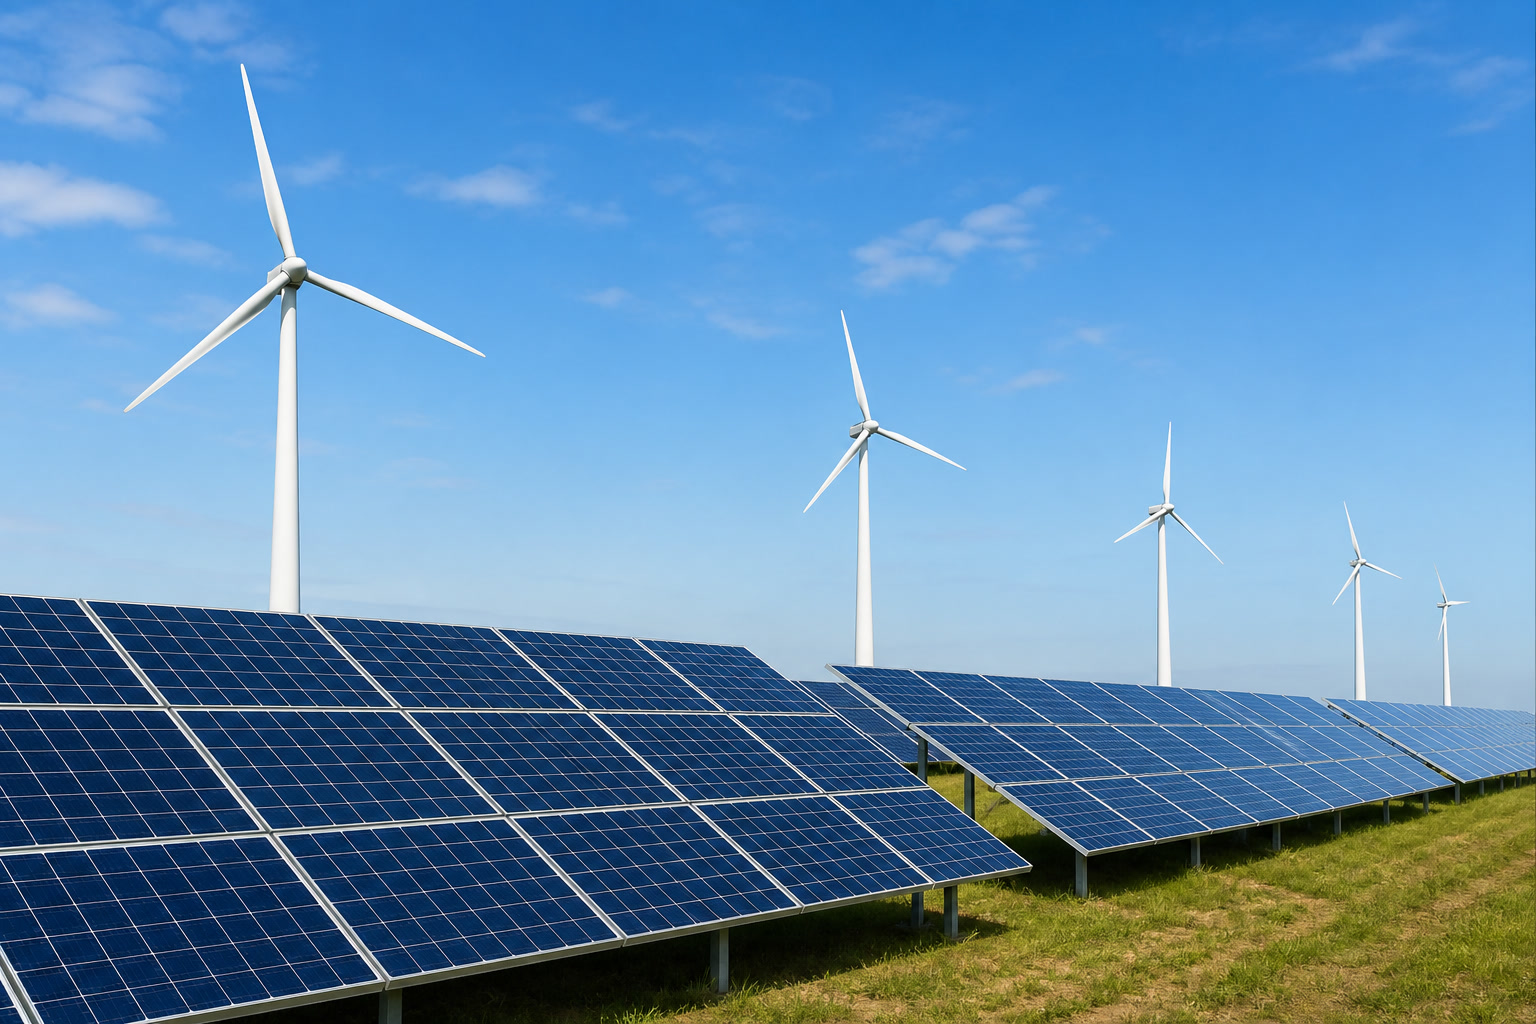
\includegraphics[width=0.55\linewidth]{images/book1/ai/g9-energy-solar-wind.jpg}

{\small Deux convertisseurs dans un même champ~: la \omterm{def:g1:light-and-shadows:source}{lumière} du Soleil devient \omterm{def:g5:everyday-energy:energy}{énergie} électrique dans les panneaux, l'\omterm{def:g2:air-around-us:air}{air} en mouvement devient \omterm{def:g5:everyday-energy:energy}{énergie} électrique dans les éoliennes.}
\end{omfigure}

\begin{remark}[Ce que «~économiser l'énergie~» veut vraiment dire]\label{rem:g9:energy-conversions:saving}
Si la conservation garde chaque \omterm{def:g9:kinetic-energy-safety:joule}{joule}, pourquoi faudrait-il
«~économiser l'\omterm{def:g5:everyday-energy:energy}{énergie}~»~? Parce que la loi préserve la
\emph{quantité}, non l'\emph{utilité}. Des réserves concentrées ---
combustible, charge, hauteur --- peuvent se dépenser en tiédeur
répandue en couche mince à travers le monde, et cette tiédeur
répandue, bien que chacun de ses \omterm{def:g9:kinetic-energy-safety:joule}{joules} survive, ne peut plus faire
marcher ni bouilloires ni trains~: la rivière est descendue. Le
problème énergétique de la civilisation n'est pas une pénurie de
\omterm{def:g9:kinetic-energy-safety:joule}{joules} --- le Soleil nous en douche des milliers de fois nos besoins
--- mais le ménagement de ceux qui sont \emph{utiles}. Cette idée,
rendue précise, est l'une des histoires les plus célèbres de la
physique~; elle attend dans les années d'université sous son nom
fameux.
\end{remark}

\section{Exercices}

\begin{exercise}[$\star$]\label{exo:g9:energy-conversions:1}
Nomme les sept formes du catalogue, chacune avec un exemple
domestique.
\end{exercise}

\begin{exercise}[$\star$]\label{exo:g9:energy-conversions:2}
Calcule $E_p$~: un seau de \qty{2}{kg} monté de \qty{10}{m}~; un
randonneur de \qty{60}{kg} au sommet d'une montée de \qty{500}{m}.
\end{exercise}

\begin{exercise}[$\star$]\label{exo:g9:energy-conversions:3}
Énonce la loi de conservation, et ce qu'elle a fait aux machines à
mouvement perpétuel de tes chapitres d'enfance.
\end{exercise}

\begin{exercise}[$\star$]\label{exo:g9:energy-conversions:4}
Audite le pendule sur une oscillation~: les comptes en haut, en bas,
et la lente dérive d'ensemble --- vers où~?
\end{exercise}

\begin{exercise}[$\star$]\label{exo:g9:energy-conversions:5}
Sers-toi de $v = \sqrt{2 g h}$~: la \omterm{def:g7:motion-average-speed:formula}{vitesse} d'entrée dans l'eau depuis
un plongeoir de \qty{5}{m} --- et pourquoi la \omterm{def:g3:measuring-mass:mass}{masse} du plongeur n'est
jamais entrée en jeu.
\end{exercise}

\begin{exercise}[$\star$]\label{exo:g9:energy-conversions:6}
Définis le \omterm{def:g9:energy-conversions:efficiency}{rendement}. Un \omterm{ex:g6:circuits-and-safety:motor}{moteur} reçoit \qty{200}{J} et livre
\qty{170}{J} de mouvement~: \omterm{def:g9:energy-conversions:efficiency}{rendement}, et sort du reste~?
\end{exercise}

\begin{exercise}[$\star$]\label{exo:g9:energy-conversions:7}
Pourquoi l'ampoule ancestrale méritait-elle assez bien le nom de
«~radiateur qui a un passe-temps~»~? Donne les deux pourcentages.
\end{exercise}

\begin{exercise}[$\star$]\label{exo:g9:energy-conversions:8}
Écris la chaîne complète de conversion de la montée du cycliste ---
du petit-déjeuner au sommet --- en nommant chaque forme et chaque
fuite.
\end{exercise}

\begin{exercise}[$\star\star$]\label{exo:g9:energy-conversions:9}
Le grand livre du barrage~: \qty{1000}{kg} d'eau tombent de
\qty{50}{m} à travers les turbines. Calcule l'$E_p$ livrée~; à
quatre-vingt-dix pour cent de conversion, l'\omterm{def:g5:everyday-energy:energy}{énergie} électrique par
tonne --- et les tonnes par seconde nécessaires pour une \omterm{def:g9:electric-power-energy:power}{puissance} de
sortie de \qty{4.4e6}{W}.
\end{exercise}

\begin{exercise}[$\star\star$]\label{exo:g9:energy-conversions:10}
Une balle de \qty{0.5}{kg} lâchée de \qty{2}{m} rebondit à
\qty{1.2}{m}. Audite le rebond~: les \omterm{def:g5:everyday-energy:energy}{énergies} avant et après, la
taille et la destination de l'écrémage --- et la hauteur de rebond
au-delà de laquelle aucun audit ne trouvera plus d'\omterm{prop:g9:kinetic-energy-safety:formula}{énergie cinétique}
ni potentielle.
\end{exercise}

\begin{exercise}[$\star\star$]\label{exo:g9:energy-conversions:11}
«~L'ascenseur convertit l'\omterm{def:g5:everyday-energy:energy}{énergie} électrique en \omterm{def:g9:energy-conversions:forms}{énergie potentielle}
avec un \omterm{def:g9:energy-conversions:efficiency}{rendement} de quatre-vingt-dix pour cent.~» Calcule l'\omterm{def:g5:everyday-energy:energy}{énergie}
électrique nécessaire pour élever une cabine de \qty{500}{kg} de
\qty{30}{m} --- et concilie les dix pour cent supplémentaires avec la
loi de conservation.
\end{exercise}

\begin{exercise}[$\star\star\star$]\label{exo:g9:energy-conversions:12}
Le pratiquant de demi-tube part au repos du bord gauche, à
\qty{4}{m} de hauteur. Prédis la \omterm{def:g7:motion-average-speed:formula}{vitesse} de passage en bas, la
hauteur atteinte à droite --- idéalement et réellement --- et esquisse
le destin à long terme du mouvement et de son \omterm{def:g5:everyday-energy:energy}{énergie}. Puis explique,
avec \cref{rem:g9:energy-conversions:saving}, pourquoi aucune poussée
au bord ne peut jamais être récupérée intégralement~: qu'a gagné le
grand livre du monde, et qu'a perdu irrémédiablement le
pratiquant~?
\end{exercise}

\section{Problème~: la commission du parc d'attractions}

\begin{problem}[{Problème du week-end --- le parc d'attractions
engage une conseillère en physique~; montagnes russes, tours et le
grand livre qui ne sait pas mentir}]\label{pb:g9:energy-conversions:1}
Les nouvelles attractions du parc doivent passer ton audit énergétique
avant le jour de l'ouverture. Prends $g = \qty{9.8}{N/kg}$~; ignore
le frottement jusqu'à ce qu'il refuse d'être ignoré.

\medskip\noindent\textbf{Partie I --- la Grande Chute.}
Un train de montagnes russes de \qty{2000}{kg} est treuillé jusqu'à un
sommet de \qty{45}{m} et lâché au repos.
\begin{enumerate}
  \item L'$E_p$ du train au sommet~?
  \item Sa \omterm{def:g7:motion-average-speed:formula}{vitesse} idéale au bas de la chute, par la formule où la
        \omterm{def:g3:measuring-mass:mass}{masse} se simplifie --- en \unit{m/s} et en \unit{km/h}~?
  \item Les concepteurs ajoutent une seconde colline de \qty{50}{m}
        juste après la chute. Oppose-lui ton veto avec le grand
        livre --- et énonce la plus haute seconde colline que le
        train idéal pourrait franchir.
  \item La \omterm{def:g7:motion-average-speed:formula}{vitesse} mesurée en bas vaut \qty{28}{m/s}, non la
        valeur idéale. Calcule les deux \omterm{prop:g9:kinetic-energy-safety:formula}{énergies cinétiques} et
        impute la différence au bon compte.
\end{enumerate}

\medskip\noindent\textbf{Partie II --- le treuil et la facture.}
\begin{enumerate}[resume]
  \item Le treuil hisse le train à son sommet en \qty{60}{s}. À
        \omterm{def:g9:energy-conversions:efficiency}{rendement} parfait, sa \omterm{def:g9:electric-power-energy:power}{puissance}~?
  \item Le treuil réel appelle \qty{20}{kW}. Son \omterm{def:g9:energy-conversions:efficiency}{rendement}~?
  \item Chaque tour part toutes les quatre minutes, dix \omterm{ex:g2:measuring-time:clock}{heures} par
        jour. L'\omterm{def:g5:everyday-energy:energy}{énergie} quotidienne du treuil en \omterm{def:g9:electric-power-energy:kwh}{kilowattheures}
        (treuil réel, compte les montées), et son coût à $0.25$
        l'\omterm{def:g6:measurement-in-science:measuring}{unité}~?
  \item Un concepteur propose de récupérer l'\omterm{def:g5:everyday-energy:energy}{énergie} d'arrivée du
        train avec un frein-générateur qui alimente le réseau ---
        «~l'attraction se paiera toute seule~!~». Audite ce rêve~:
        quelle fraction pourrait revenir de façon réaliste, et
        quelle loi interdit le cercle complet~?
\end{enumerate}

\medskip\noindent\textbf{Partie III --- la tour de chute libre et le
rapport.}
La tour de \qty{60}{m} laisse tomber une nacelle de \qty{500}{kg}
dans des freins magnétiques à \qty{10}{m} du sol.
\begin{enumerate}[resume]
  \item \omterm{def:g7:motion-average-speed:formula}{Vitesse} à l'entrée de la zone de freinage (une chute idéale
        de \qty{50}{m})~?
  \item \omterm{def:g5:everyday-energy:energy}{Énergie} que les freins doivent mettre à la retraite, et où
        l'induction l'envoie. (Ces freins sont les cousins du
        chapitre de l'\omterm{def:g9:alternator:alternator}{alternateur} --- des tourbillons de courant
        induit qui échauffent le métal.)
  \item Les passagers hurlent qu'ils étaient «~en apesanteur~»
        pendant la chute. À partir de l'idée des compagnons de
        chute du chapitre sur la \omterm{def:g9:gravitation:gravitation}{gravitation}, tranche cette
        affirmation en une phrase.
  \item Signe le rapport de la commission~: trois phrases ---
        l'échange dont vivent les montagnes russes, la loi à
        laquelle toutes les attractions ont obéi, et le compte qui
        les a toutes discrètement taxées.
\end{enumerate}
\end{problem}
